\section{Introduction}
\begin{frame}{Introduction}


\justifying{
\begin{itemize}
  \item We were approached by a large tech company for help with their threat alert system. 
\begin{itemize}
\item They have a mature insider threat stack.
\item Includes multiple models, IDS, and threat hunting methods.
\end{itemize}
\pause
\item They receive too many alerts for their security analysts to go through manually, resulting in alert fatigue.
\end{itemize}}

\begin{center}

\includegraphics[scale=0.25]{analyst.jpg}
\end{center}
\end{frame}


\begin{frame}{The data}
  \begin{itemize}
    \item What does the data look like? 
    
    \pause 
    
    \item The company's system flags suspicious events and records data about the event and the entities involved.
  \end{itemize}
  
  \pause
  
  \begin{center}
  	Sample Event:
  	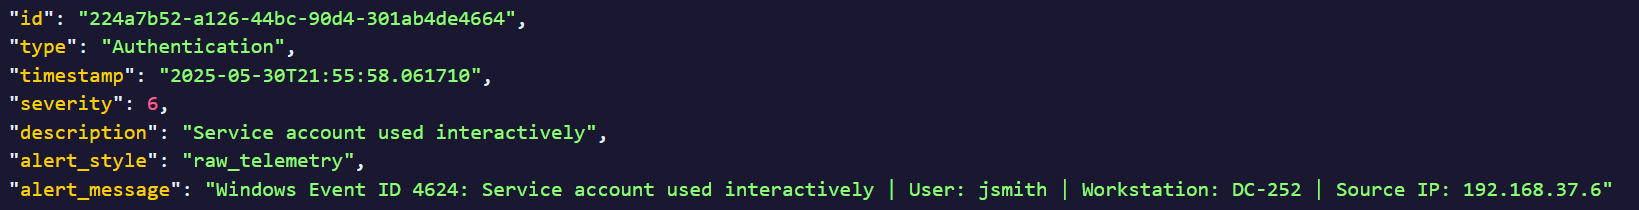
\includegraphics[scale=0.4]{event.png}
  \end{center}
  
  \pause
  
  \begin{center}
  	Sample Entity: \\
  	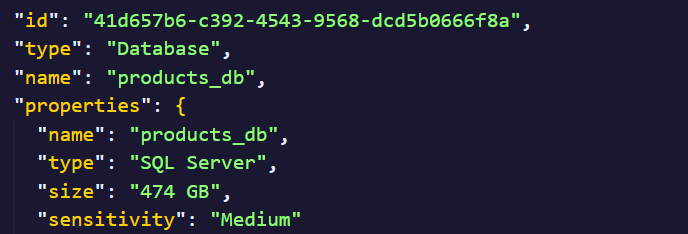
\includegraphics[scale=0.4]{entity.png}
  \end{center}
  
  \pause
  
  \begin{center}
  	Sample Relationship: \\
  	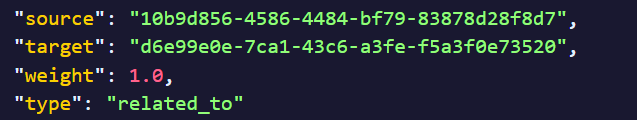
\includegraphics[scale=0.4]{relationship.png}
  \end{center}
\end{frame}

\begin{frame}{Business Needs}
	\begin{itemize}
		\item The data consists of hundreds of events, entities, and relationships between them.
		
		\item This is too much for the analyst to go through every week.
		
		\pause
		
		\item Our goal is to clump events together into potential attack scenarios and provide the analyst with a (much smaller) list of events to look into manually.
	\end{itemize}
	
	\pause
	
	\begin{center}
	
\includegraphics[scale=0.1]{analyst_happy.png}
	\end{center}
\end{frame}

\begin{frame}{Outcomes}
	\begin{itemize}[itemsep = 12 pt, topsep=48 pt]
		\item Success will be measured by our ability to make the analyst's job easier.
		
		\pause
		
		\item Saving the company money and resources, mostly in human-hours, and allowing the analyst to spend more time on other projects.
		
		\pause
		
		\item While also hopefully being able to more reliably alert the company to malicious attack scenarios.
	\end{itemize}
\end{frame}
